\begin{history}

    % \subsection{1925-1950}

    In diesem Vierteljahrhundert machte die Musikgesellschaft auf musikalischem
    Gebiet grosse Fortschritte. In diese Zeitspanne fallen die Besuche der
    Musikanlässe ‘von Hochdorf, Rickenbach, Wolhusen, Willisau, 'Ebikon, Rain
    und an das Eidg. Musikfest in St. Gallen. Die Teilnahme an diesen Festen,
    welche an die Direktion und an die Bläser hohe Anforderungen stellte, liess
    erkennen, dass der Verein gewillt war, eine höhere Stufe zu erreichen und
    nach Möglichkeit diese zu halten. Die vermehrte und auf Blasmusik
    zugeschnittene Literatur verlangte intensivere Probenarbeit. Tüchtiges und
    zielbewusstes Schaffen brachte der Musikgesellschaft Hildisrieden Lorbeeren
    ein, auf die sie sicher stolz sein konnte,

    Ausser dem Besuch von Musikfesten fand der Verein noch Zeit, an
    verschiedenen Veranstaltungen mitzuwirken. So treffen wir ihn 1929 am
    Festzug des Schweiz. Katholikentages in Luzern, als Festmusik an der
    Pferde-Springkonkurrenz und 1943 an der Vereranentagung des
    Kantonal-Schützenverbandes in Hildisrieden.

    An der Generalversammlung von 1932 wurde der Vorstand für eine weitere
    Amtsdauer (von 2 Jahren) bestätigt:

    Präsident: Josef Disler, Dorf Vize-Präsident: Alois Estermann, Traselingen
    Aktuar: Karl Estermann, Traselingen Kassier: Heinrich Estermann, Oele
    Beisitzer: Leo Erni, Wirt zum Kreuz. Jakob Estermann, Dorf Dirigent: Alois
    Estermann, Traselingen


    Eine besondere Anerkennung sei hier kurz der Vereinsführung gezollt. Im
    Vorstand treffen wir bis 1945 keinen Wechsel von grosser Bedeutung. Man fand
    stets wieder die geeignete Person, um entstandene Lücken zu füllen. Josef
    Disler, welcher der Musikgesellschaft volle 17 Jahre vorstand, wurde zum
    Dank für die geleisteten treuen Dienste zum Ehrenpräsidenten ernannt.

    Dass in einer Uniform der Musikant erst so recht zur Geltung kommt, ist
    altbekannt. Die Finanzierung der Neu-Uniformierung konnte die Kasse nicht
    verkraften. Durch eine Sammelaktion wurde der benötigte Betrag aufgebracht.

    Das Jahr 1939 brachte der Musikgesellschaft etwas Ungewolltes. Die in diesem
    Jahre ausgebrochene Maulund Klauenseuche verhinderte einen geordneten.
    Probenbetrieb. Aber der im September entfachte Zweite Weltkrieg, der die
    Grosszahl der Mitglieder an die Grenze rief, wirkte nicht weniger hemmend.
    Die Musikgesellschaft hatte die Ehre, damals schon eine stattliche Zahl
    Militärtrompeter zu stellen, die während der langen Aktivdienstzeit
    musikalische Weiterbildung genossen.

    Solange die Musikgesellschaft bestand, fehlte sie nie an einer kirchlichen
    Feier. Am Fronleichnamstag 1940 aber waren so viele Musikanten an der
    Grenze, dass der Verein ausserstande war, die Prozession würdig zu
    gestalten. Das Spiel des Inf Reg 86, das in Hildisrieden einquartiert war,
    gab dem Allerheiligsten das Geleit und bekundete so die Verbundenheit von
    Volk und Armee.

    Im Frühjahr 1945 nahm der mörderische Krieg, der so viele Tränen fliessen
    liess, endlich ein Ende. Der denkwürdige 8. Mai wurde zum
    Waffenstillstandstag erklärt. Mit dem Wegfall des Aktivdienstes begann
    wieder ein regelmässiges Vereinsleben mit Probenbetrieb in alter Form. Der
    neu gewählte Präsident, Josef Rüttimann, wurde allen Aktiven ein Vorbild.

    1949 war für die Musikgesellschaft ein Jubeljahr. Der fünfundsiebzigste
    Geburtstag wurde gebührend gefeiert.

    \subsubsection{Erste Uniform 1933}

    Die Musikgesellschaft hat an der Generalversammlung vom 28. März 1933
    einstimmig beschlossen, eine Uniform anzuschaffen. Da sämtliche Musikvereine
    der Nachbarschaft schon längst uniformiert waren, begrüsste man diesen
    einmütigen Beschluss. Um die nötigen Geldmittel zu beschaffen, sollte ca.
    1/3 die Vereinskasse leisten. Der Rest von rund Fr. 2000.— musste durch eine
    Sammlung aufgebracht werden. Das Bekleidungshaus Stutz in Hochdorf erhielt
    am 22. Mai 1933 den Auftrag. Die Uniform umfasst eine schwarze Hose, einen
    grünen Rock, eine Mütze und eine Musikschnur. Preis Fr. 126.—. Dazu kam noch
    eine Musiktasche aus feinstem Rindsleder, vom Aktivmitglied Hans Winiger,
    Sattler, angefertigt. Diese Tasche kostete Fr. 12.—. Die ganze Uniformierung
    betrug somit Fr. 3036.—.

    Was man schon längst für angezeigt hielt, und dem Fortschritt der Zeit
    entsprach, war nun Tatsache geworden. Am Abend des 20. August leitete ein
    Konzert im Löwensaal die Einweihung ein. Präsident Josef Disler dankte allen
    Spendern, die trotz Krisenzeiten eine offene Hand hatten und betonte, dass
    das ein Ehrentag für die Musikanten sei. Die Uniformierung fiel mit dem
    sechzigjährigen Bestehen des Vereins zusammen.

\end{history}

\groupphoto{0.93}{0.8}{./chap/1925-1950/MGH-1934.jpg}
{\emph{1934}\\
    Sitzend:\\
    Kramis Alois, Fischer Josef, Portmann Josef, Estermann Heinrich, Erni Leo,
    Troxler Kaspar\\
    1. Reihe:\\
    Disler Josef, Estermann Robert, Zwinggi Jakob, Winiger Hans, Estermann
    Alois, Dirigent, Estermann Karl, Suter Kaspar, Suter Jakob, Fleischlin
    Kaspar, Estermann Jakob\\
    2. Reihe:\\
    Estermann Josef, Rüttimann Josef, Troxler Hans, Troxler Alfred, Küng Emil\\
    3. Reihe:\\
    Jutz Hans, Estermann Josef, Suppiger Hans }
{fig:mgh-1934}

\begin{figure}[!htbp]
    \centering
    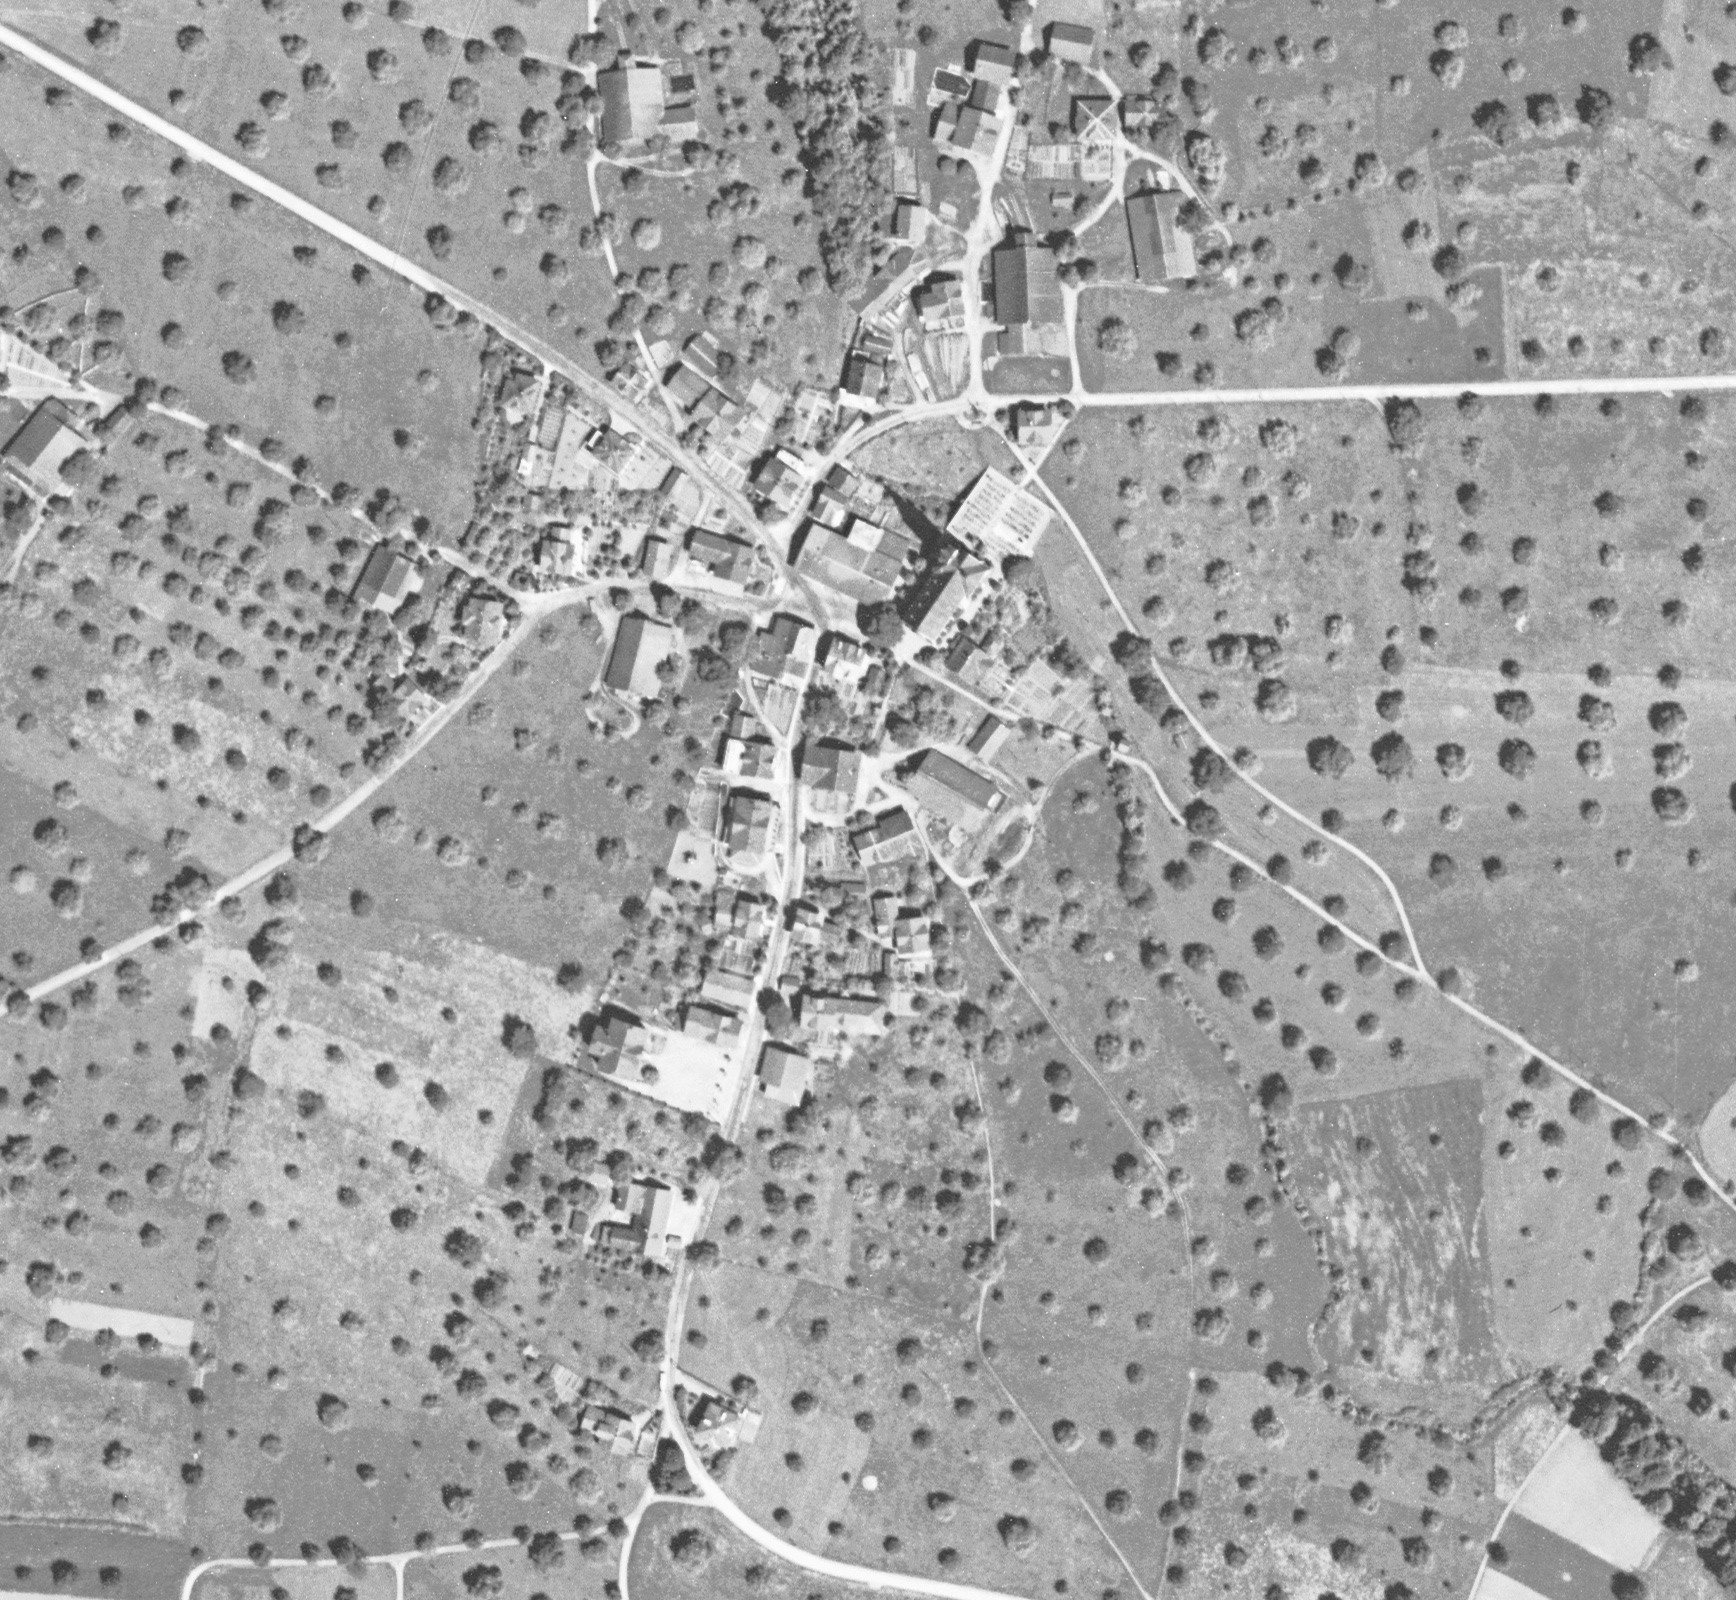
\includegraphics[height=\textheight,keepaspectratio]{./Dorf-Bilder/Luftaufnahme-1931.jpg}
    \caption{Luftaufnahme 1931}
\end{figure}

\begin{figure}[ht]
    \centering
    \def\theight{0.43}
    \subfloat[Löwen mit Tankstelle]{%
        \includegraphics[height=\theight\textheight,keepaspectratio]{./Dorf-Bilder/Alter-Löwen.jpg}%
    }\hfil
    \subfloat[Fasnacht vor der Kreuzscheune]{%
        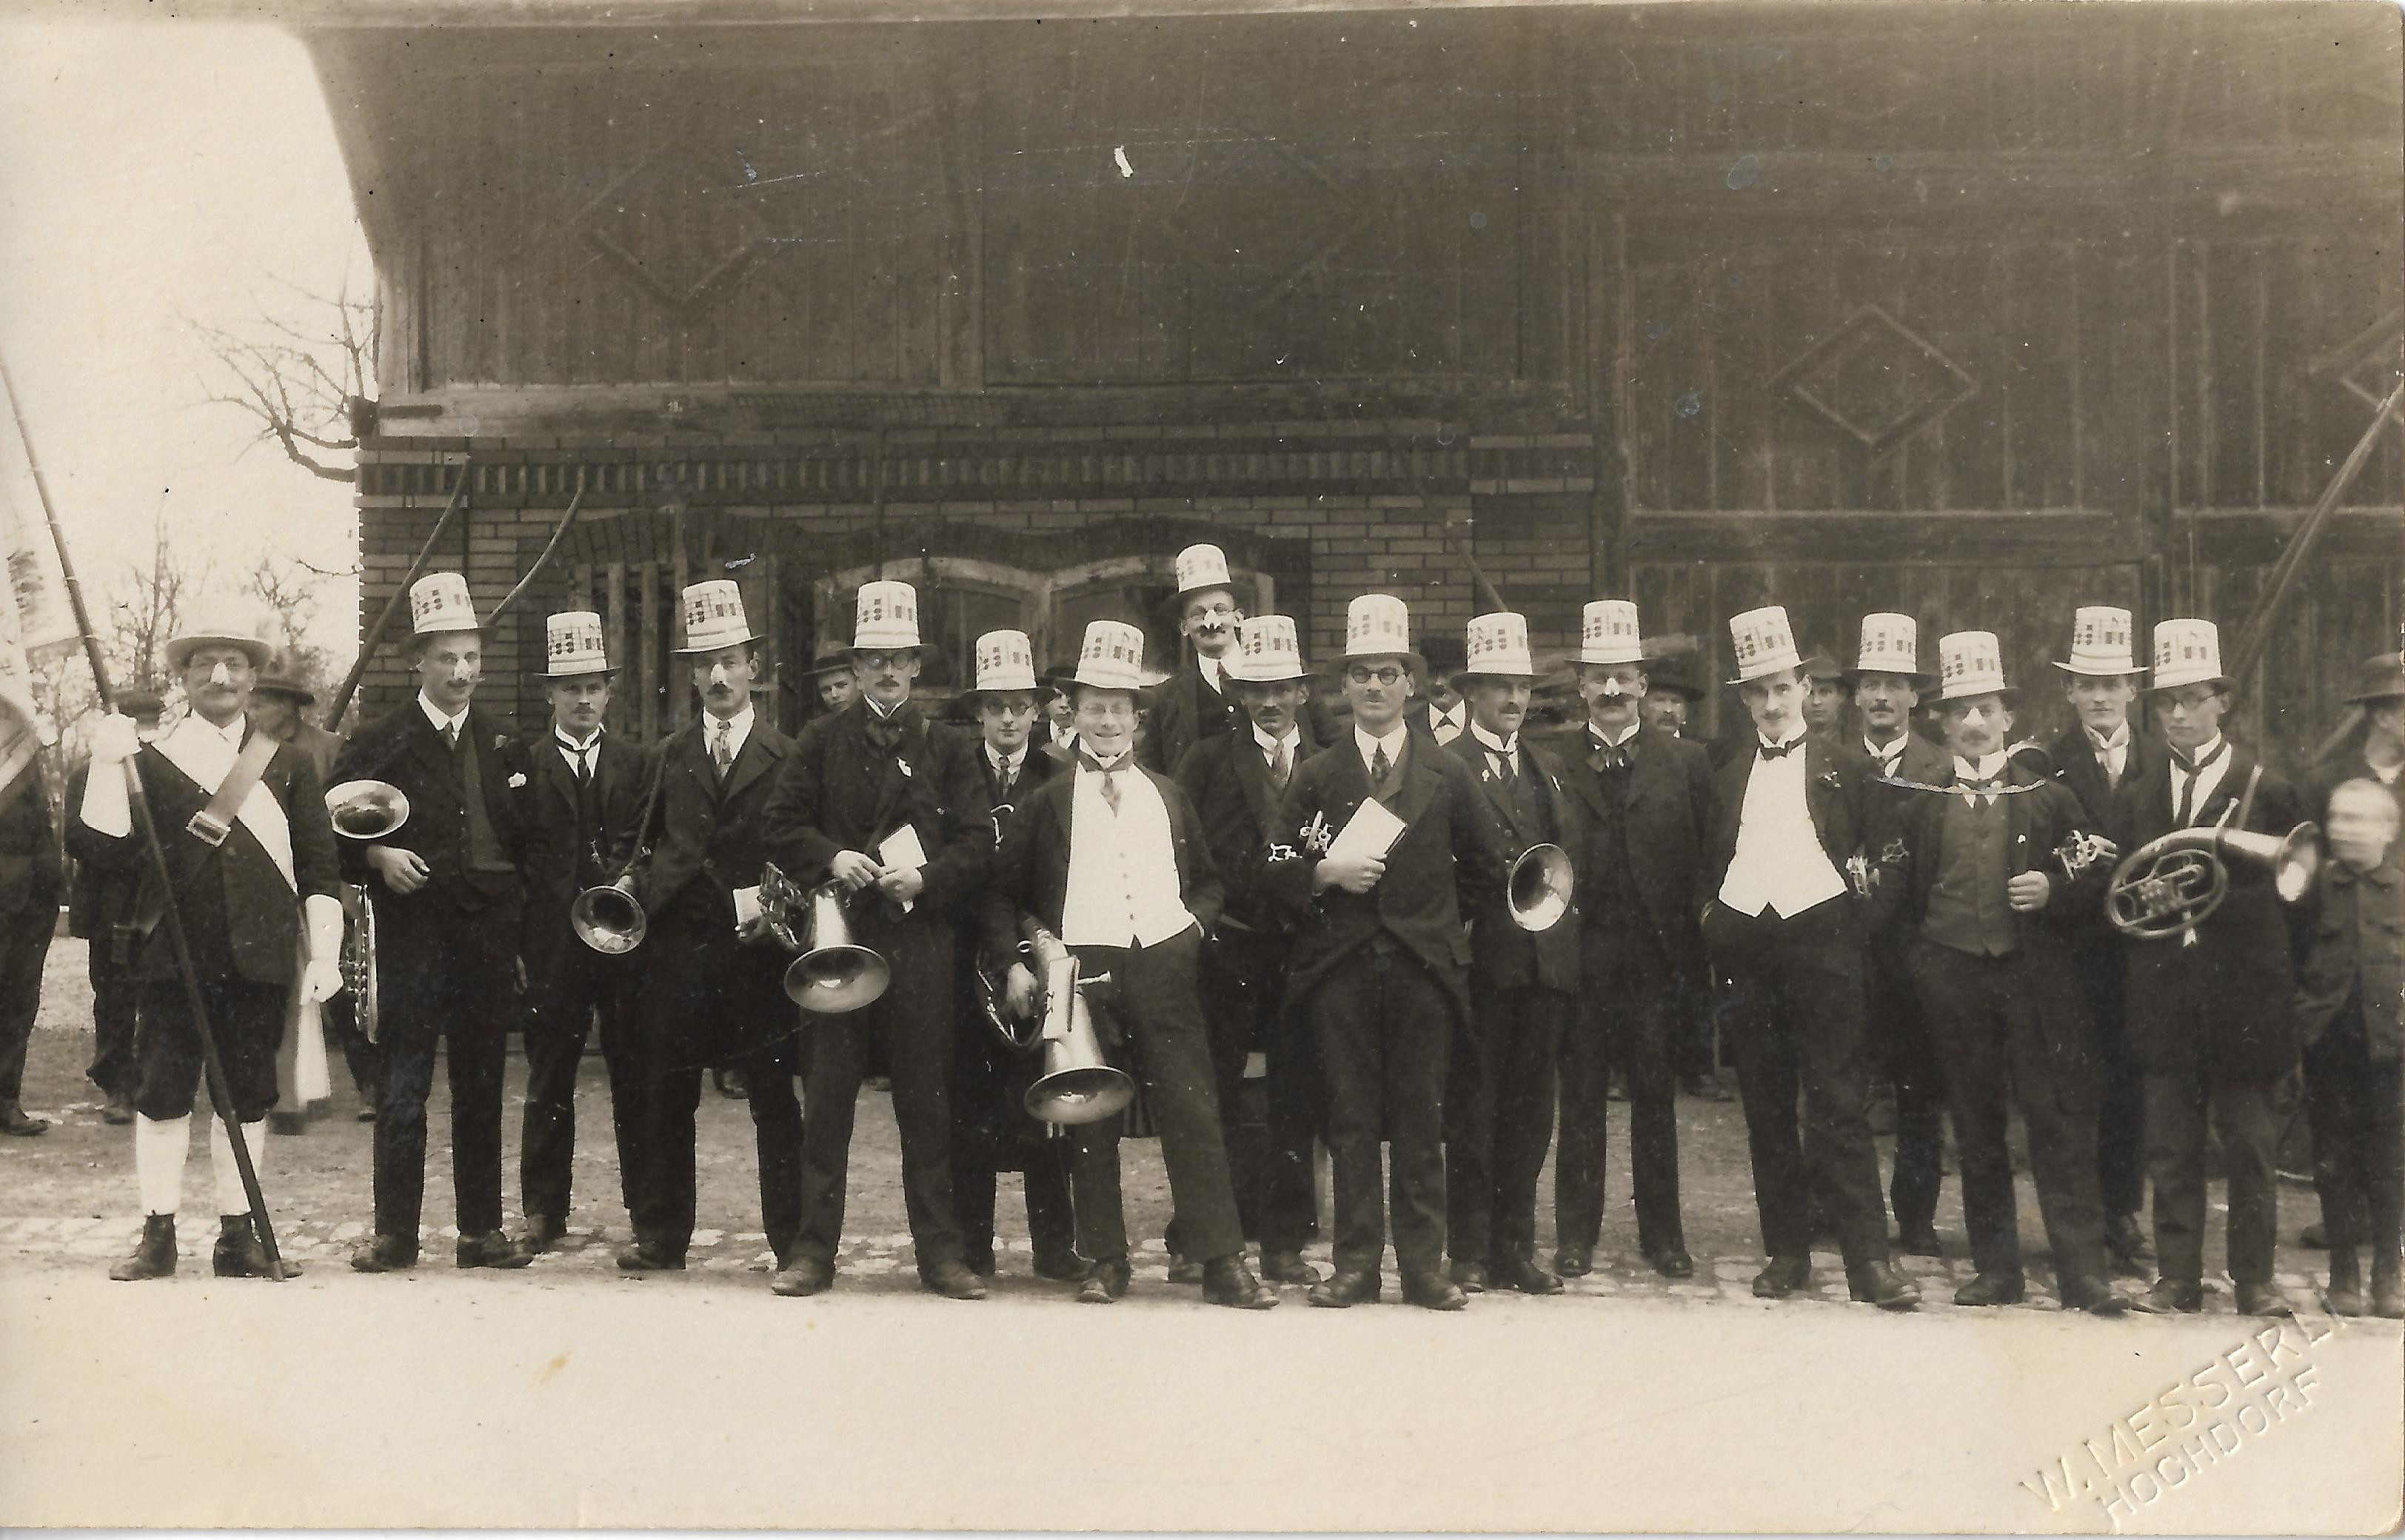
\includegraphics[height=\theight\textheight,keepaspectratio]{./chap/1925-1950/Fasnacht-vor-Kreuz-Scheune-1930er.jpg}%
    }\\
    \subfloat[Fasnacht in den 1940ern]{%
        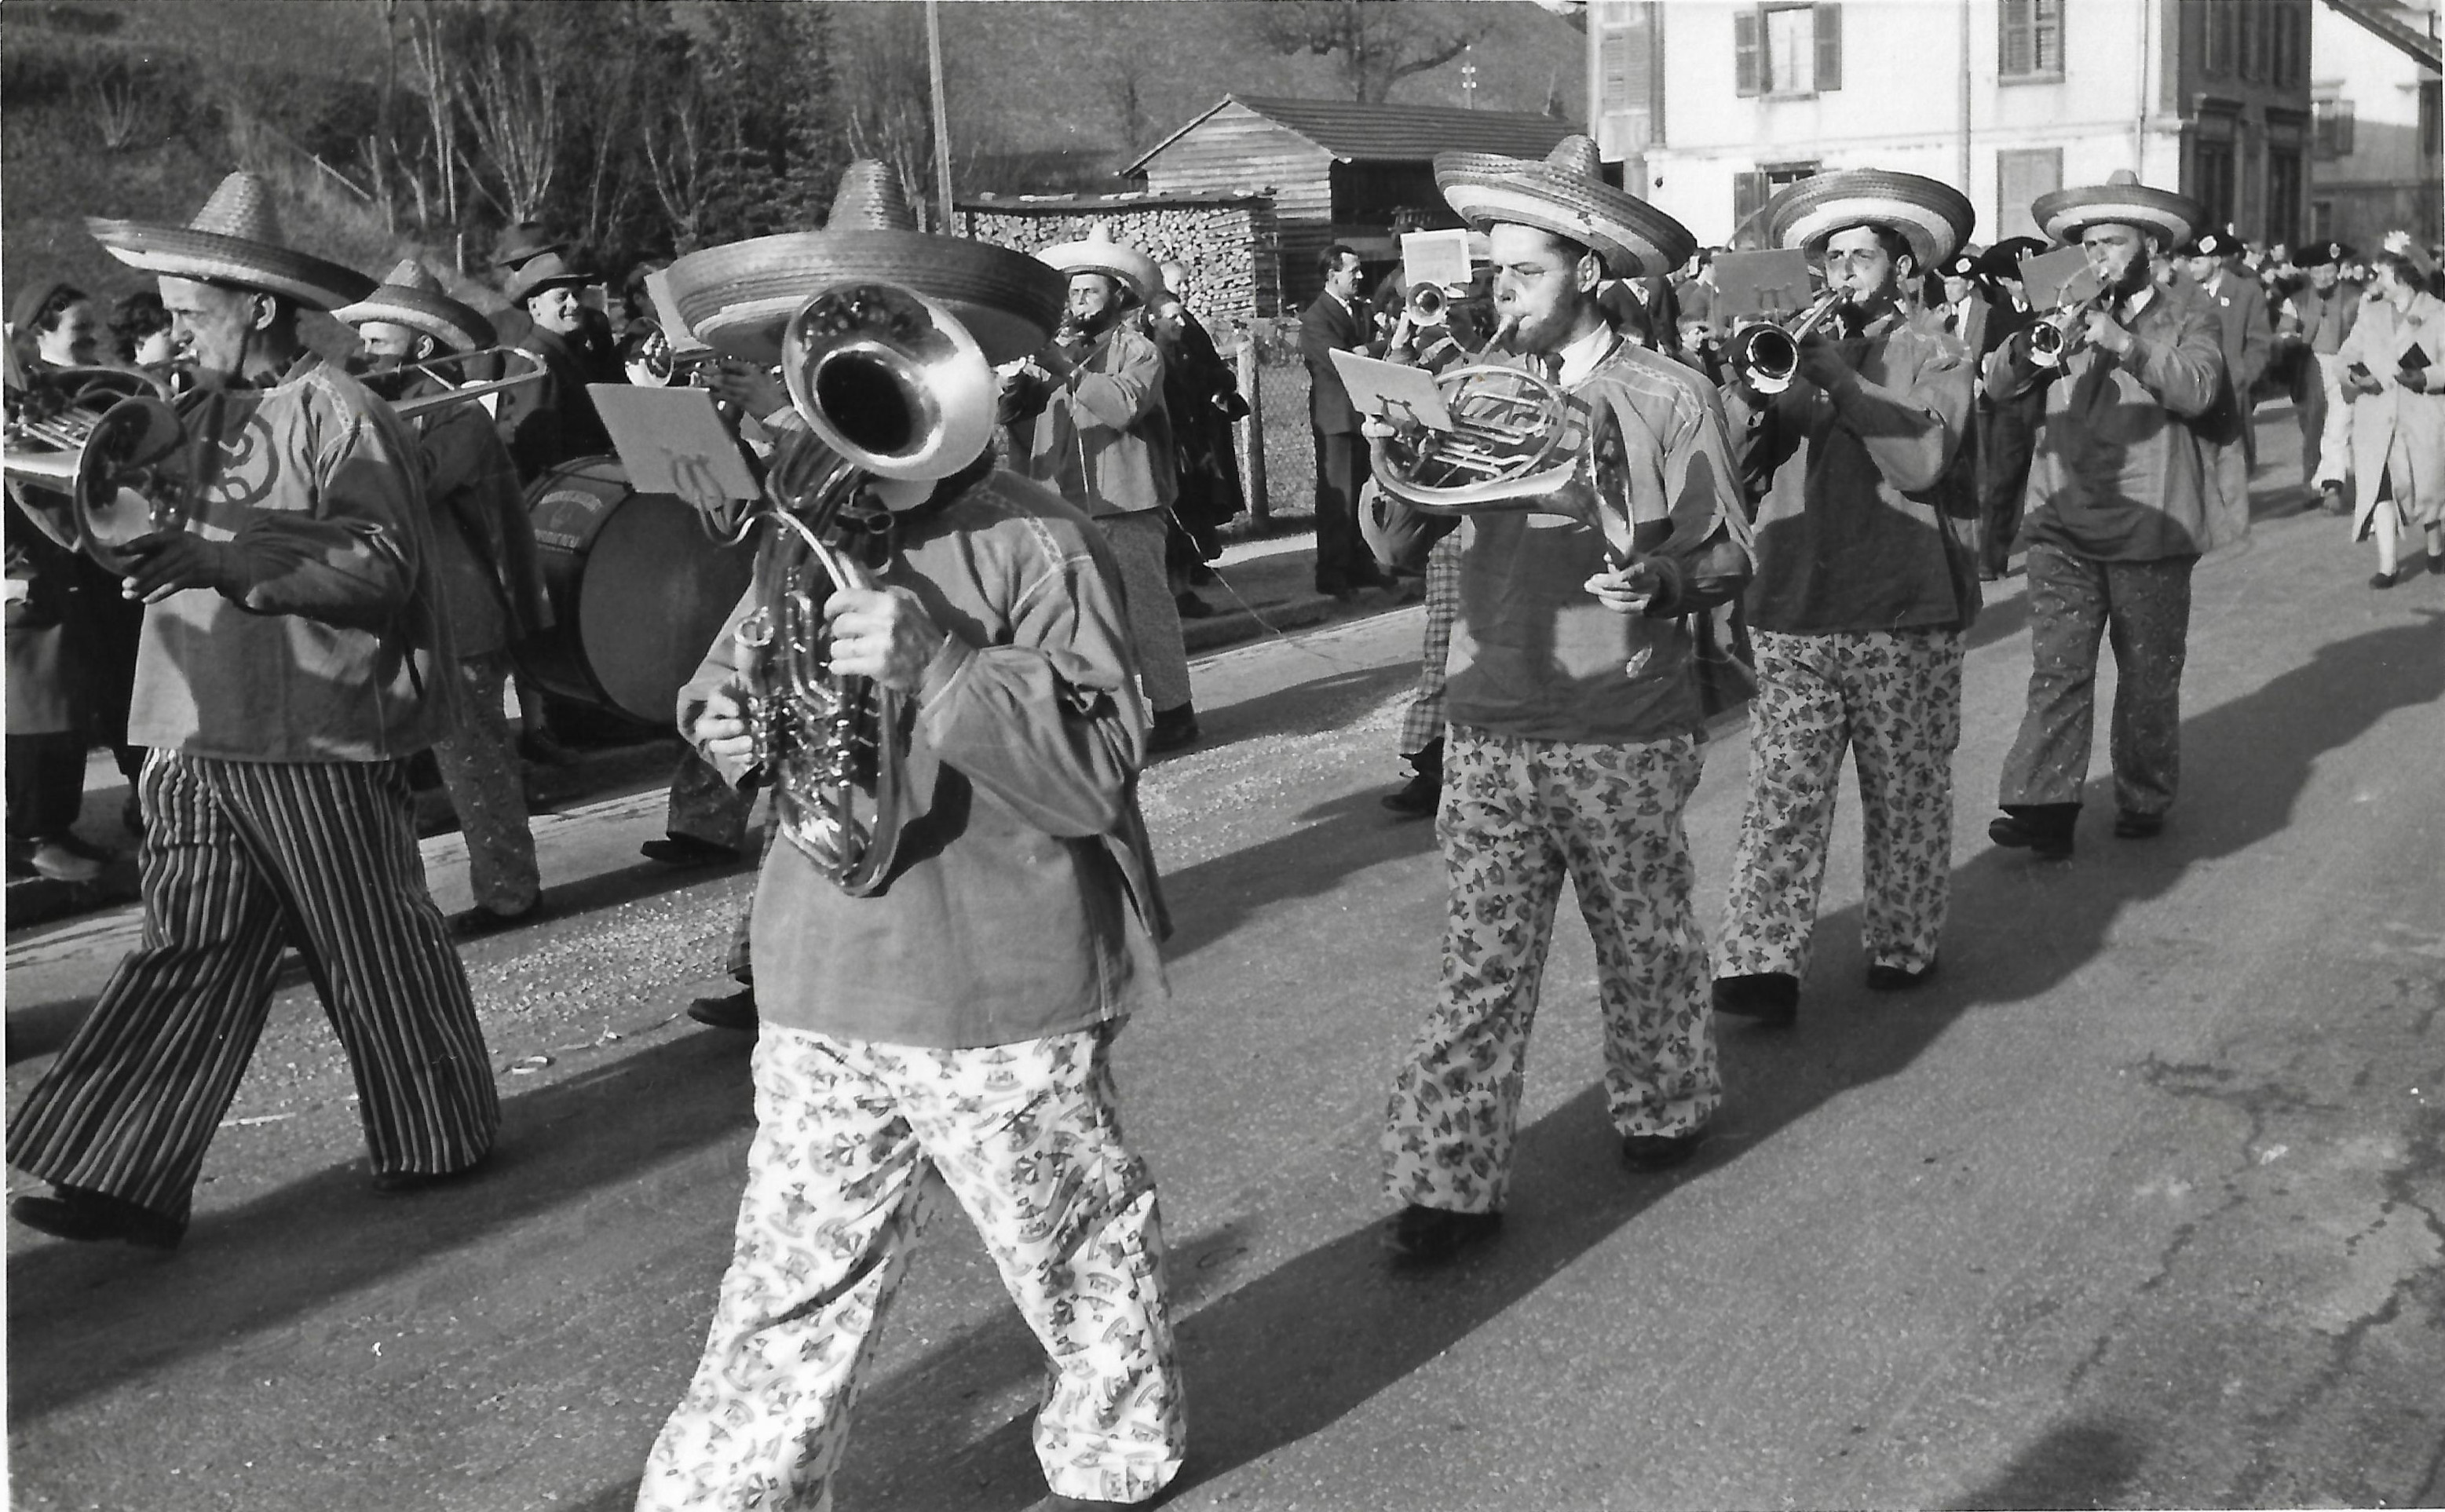
\includegraphics[height=\theight\textheight,keepaspectratio]{./chap/1925-1950/Fasnacht-1946.jpg}%
    }\hfil
    \subfloat[Weisser Sonntag 1946]{%
        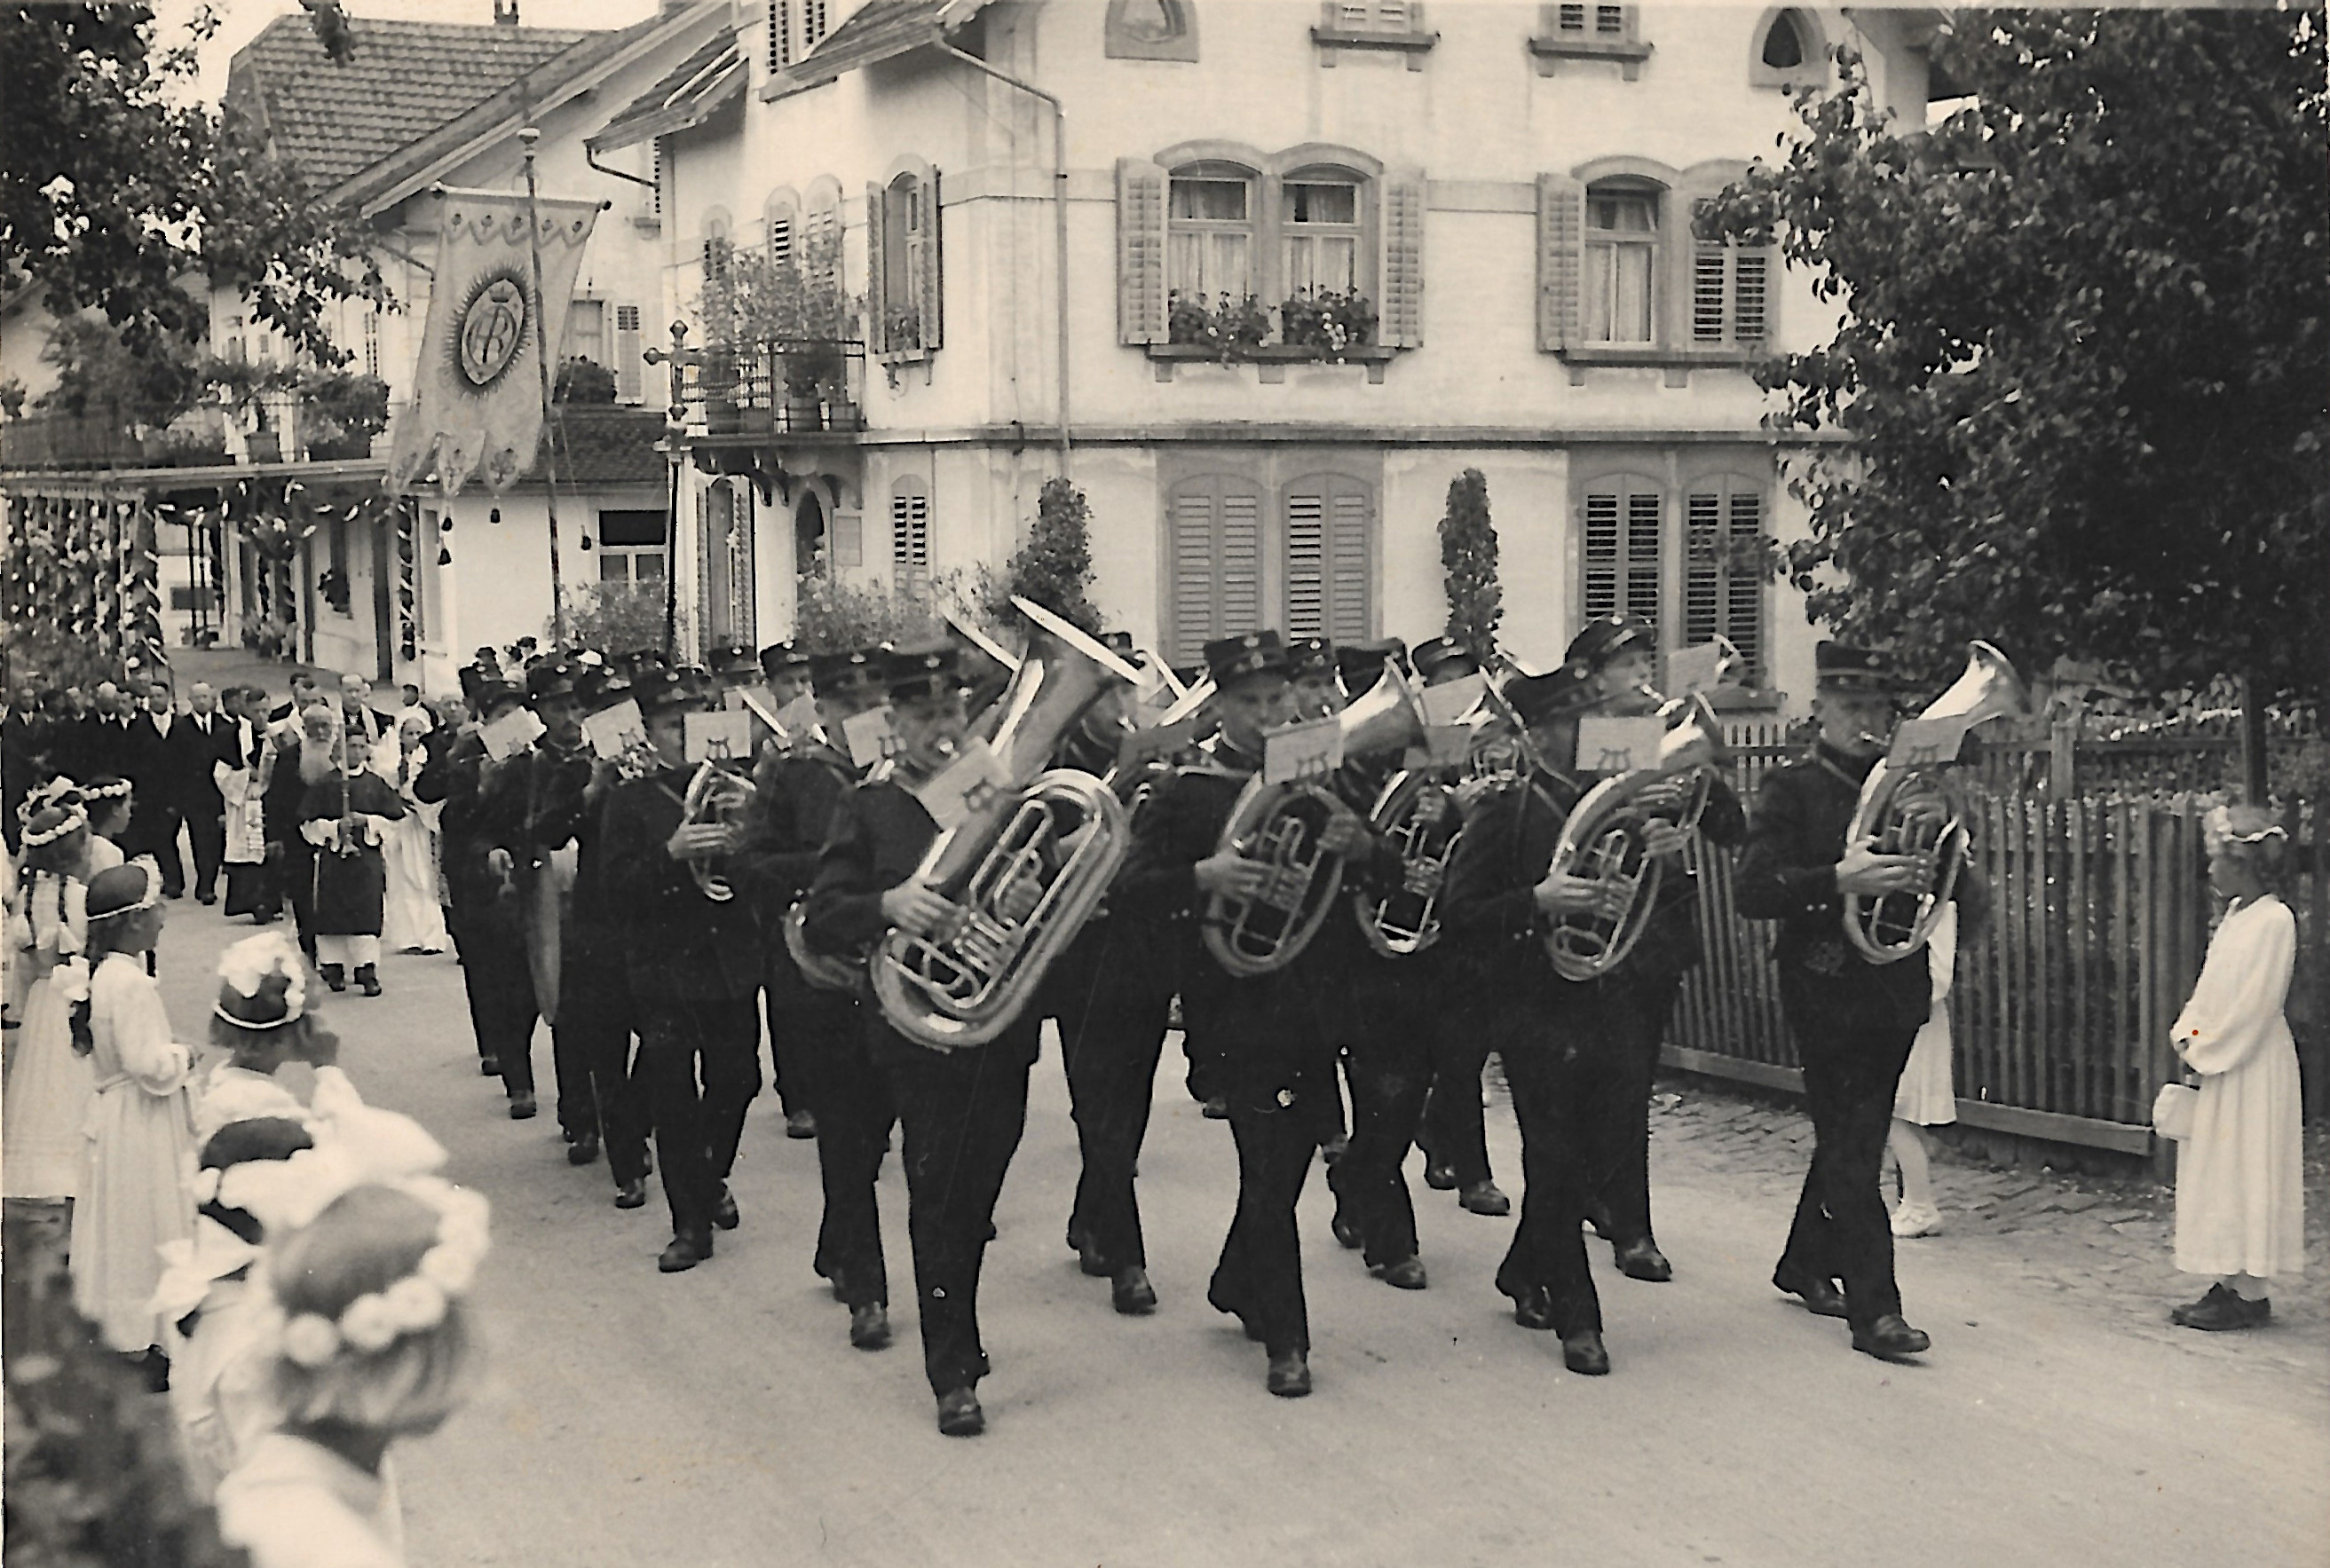
\includegraphics[height=\theight\textheight,keepaspectratio]{./chap/1925-1950/Weisser-Sontag-1946.jpg}%
    }
\end{figure}